
\renewcommand{\arraystretch}{1.5} % Default value: 1

%%%%%%%%%%%%%%%%%%%%%%%%%%%%%%%%%%%%%
\section{Introduction}
Optical fibres play a crucial role in modern communication systems due to their ability to transmit information efficiently using light. In this experiment, we study the propagation of laser light through optical fibres and analyse the quality and quantity of information carried by single-mode and multimode fibres. The working principle of optical fibres is based on total internal reflection, where light is guided through a core of higher refractive index surrounded by a lower refractive index cladding. By coupling laser light into different types of fibres and observing their output intensity distributions, we investigate how modal propagation affects signal quality. Multimode fibres support multiple propagation paths, leading to distortion and reduced coherence, whereas single-mode fibres allow only a single propagation mode, resulting in a well-defined Gaussian intensity profile. Additionally, parameters such as numerical aperture and coupling efficiency are examined to understand their influence on light transmission. This experiment thus provides insight into the fundamental physics governing optical fibre communication and highlights the differences in performance between single-mode and multimode systems.
%%%%%%%%%%%%%%%%%%%%%%%%%%%%%%%%%%%%%
\section{Objective}
The objective of this experiment is to study the propagation of laser light through optical fibres based on the principle of total internal reflection, and to analyse their effectiveness as carriers of information. The experiment aims to compare both the quantity and quality of information transmitted through single-mode and multimode optical fibres by measuring output power and examining the intensity distribution of the emerging light. It also seeks to understand the role of numerical aperture and coupling conditions in determining transmission efficiency. Furthermore, the experiment involves observing the differences in mode propagation, where multimode fibres support multiple modes leading to distortion, while single-mode fibres produce a well-defined Gaussian profile.
%%%%%%%%%%%%%%%%%%%%%%%%%%%%%%%%%%%%%
\section{Equipment Required}
The following apparatus are required for this experiment:
\begin{itemize}
    \item Red Diode laser ($650 \ nm$)
    \item Power supply
    \item Silvered mirrors
    \item Precision adjustable kinematic mounts for mirrors
    \item Optical table
    \item Fibre-optic coupler with aspheric lens on $x-y$ translation stage
    \item Two optical fibres: multimode, 600–800 nm single-mode
    \item Photodiode detector
\end{itemize}
%%%%%%%%%%%%%%%%%%%%%%%%%%%%%%%%%%%%%
\section{Theory}
\subsection{Structure and Working of Optical Fibre}

An optical fibre is a cylindrical dielectric waveguide consisting of a central \textbf{core} surrounded by a \textbf{cladding}. The refractive index of the core ($n_1$) is slightly higher than that of the cladding ($n_2$), i.e., $n_1 > n_2$. This refractive index difference is essential for guiding light through the fibre via total internal reflection.

When light is launched into the fibre within a certain range of angles (defined by the acceptance angle), it undergoes repeated total internal reflections at the core--cladding interface and propagates along the fibre with minimal loss. The efficiency of light propagation depends on proper alignment and coupling of the input beam into the fibre core. 

Depending on the core diameter and operating wavelength, optical fibres can be classified into \textbf{single-mode} and \textbf{multimode} fibres. In single-mode fibres, only the fundamental mode propagates, resulting in a well-defined Gaussian intensity profile and minimal dispersion. In contrast, multimode fibres support multiple propagation modes, leading to modal dispersion and distortion of the transmitted signal.

Thus, optical fibres serve as efficient carriers of information, where the transmitted optical power represents the quantity of information, and the spatial intensity distribution of the output beam represents its quality.


\begin{figure}[H]
    \centering
    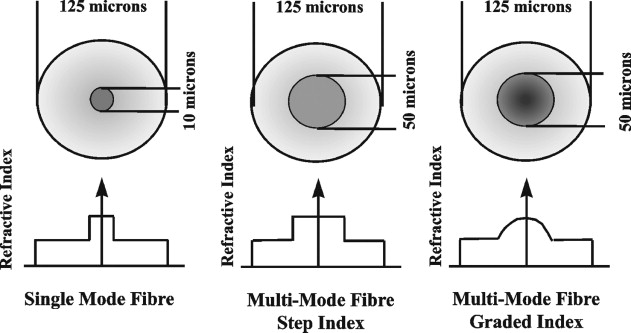
\includegraphics[width=0.7\linewidth]{Image/multi_single.jpg}
    \caption{Single and Multimode Optical Fibre}
    \label{fig:single_multi}
\end{figure}


\subsection{Total Internal Reflection}

Optical fibres operate on the principle of \textbf{total internal reflection (TIR)}. When light travels from a medium of refractive index $n_1$ to a medium of lower refractive index $n_2$ ($n_1 > n_2$), Snell’s law gives:
\begin{equation}
n_1 \sin \theta_1 = n_2 \sin \theta_2
\end{equation}
As the angle of incidence $\theta_1$ increases, the angle of refraction $\theta_2$ also increases and reaches $90^\circ$ at the \textbf{critical angle} $\theta_c$, defined by:
\begin{equation}
\sin \theta_c = \frac{n_2}{n_1}
\end{equation}
For $\theta_1 \geq \theta_c$, no refraction occurs and the entire light is reflected back into the denser medium. This phenomenon is called total internal reflection. 

An optical fibre consists of a core of refractive index $n_1$ surrounded by a cladding of refractive index $n_2 < n_1$. Light entering the fibre undergoes repeated total internal reflections at the core--cladding interface and is guided along the fibre.

\subsection{Numerical Aperture and its Derivation}

The \textbf{numerical aperture (NA)} defines the light-gathering ability of an optical fibre. It is given in terms of the maximum acceptance angle $\theta_{a}$ as:
\begin{equation}
NA = n \sin \theta_{a}
\end{equation}
To derive NA, consider a ray entering the fibre from a medium of refractive index $n$ at an angle $\alpha$. At the fibre entrance, Snell’s law gives:
\begin{equation}
n \sin \theta_{a} = n_1 \sin \theta
\end{equation}
For total internal reflection at the core--cladding interface, the limiting condition is:
\begin{equation}
\sin \theta_c = \frac{n_2}{n_1}
\end{equation}
From geometry,
\begin{equation}
\theta = 90^\circ - \theta_c \Rightarrow \sin \theta = \cos \theta_c
\end{equation}
Thus,
\begin{equation}
\cos \theta_c = \sqrt{1 - \sin^2 \theta_c} = \sqrt{1 - \left(\frac{n_2}{n_1}\right)^2}
\end{equation}
Substituting into Snell’s law:
\begin{equation}
n \sin \theta_{a} = n_1 \sqrt{1 - \left(\frac{n_2}{n_1}\right)^2}
\end{equation}
Simplifying,
\begin{equation}
n \sin \theta_{a} = \sqrt{n_1^2 - n_2^2}
\end{equation}
Therefore,
\begin{equation}
\boxed{NA = \sqrt{n_1^2 - n_2^2}}
\end{equation}
For air ($n = 1$), $NA = \sin \theta_{a}$. Only rays entering within this acceptance cone are guided through the fibre. 

\begin{figure}[H]
    \centering
    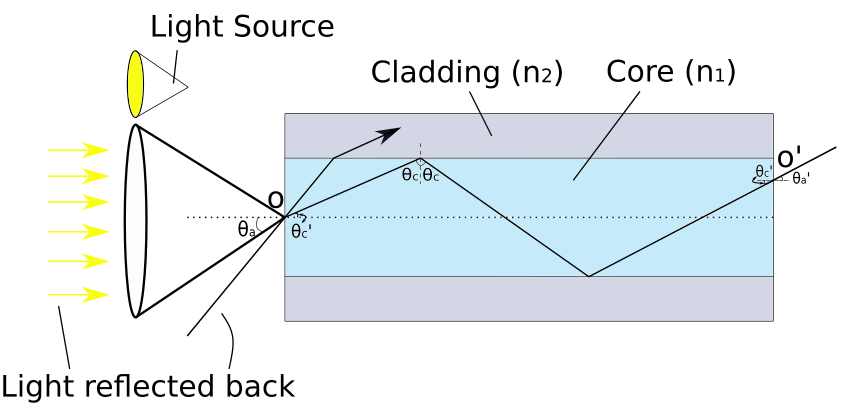
\includegraphics[width=0.7\linewidth]{Image/fibre_structure.PNG}
    \caption{Structure of the Optical Fibre}
    \label{fig:fibre_struct}
\end{figure}
\subsection{Paraxial Wave Approximation and Hermite-Gaussian Modes}
To understand we are starting with a general form of the electric field

\begin{equation}
E(x,y,z) = U(x,y,z) e^{i(kz - \omega t)} + c.c.
\end{equation}
Assume $U(x,y,z)$ is a slowly varying function of $z$. Now from Helmholtz equation:
\begin{equation}
\nabla^2 E + k^2 E = 0
\end{equation}
Now,
$$
\frac{\partial^2 E}{\partial x^2} = \frac{\partial^2 U}{\partial x^2} e^{ikz}
$$

$$
\frac{\partial E}{\partial z} = \left( \frac{\partial U}{\partial z} + ikU \right) e^{ikz}
$$

$$
\frac{\partial^2 E}{\partial z^2}
= \left( \frac{\partial^2 U}{\partial z^2} + 2ik \frac{\partial U}{\partial z} - k^2 U \right) e^{ikz}
$$
Substituting into Helmholtz equation:
\begin{align}
\nabla^2 E + k^2 E &= 0 \\
\Rightarrow \frac{\partial^2 U}{\partial x^2}
+ \frac{\partial^2 U}{\partial y^2}
+ \frac{\partial^2 U}{\partial z^2}
+ 2ik \frac{\partial U}{\partial z} &= 0
\end{align}

Now using \textbf{Slowly Varying Envelope Approximation} or \textbf{Paraxial Approximation}

\begin{equation}
\left| \frac{\partial^2 U}{\partial z^2} \right| \ll
\left| k \frac{\partial U}{\partial z} \right|
\ll |k^2 U|
\end{equation}
Hence, neglect $\frac{\partial^2 U}{\partial z^2}$:

\begin{equation}
\nabla_\perp^2 U + 2ik \frac{\partial U}{\partial z} = 0
\end{equation}
This is the \textbf{Paraxial Wave Equation}.
Now take the ansatz (Gaussian form)

\begin{equation}
U = A(z) \exp \left( i k \frac{x^2 + y^2}{2q(z)} \right)
\end{equation}

Now compute derivatives:

$$
\frac{\partial U}{\partial x}
= A(z) \frac{ikx}{q(z)} \exp \left( i k \frac{x^2 + y^2}{2q(z)} \right)
$$

$$
\frac{\partial^2 U}{\partial x^2}
= \left[ A(z) \frac{ik}{q(z)} - A(z) \frac{k^2 x^2}{q^2(z)} \right]
\exp \left( i k \frac{x^2 + y^2}{2q(z)} \right)
$$

$$
\frac{\partial U}{\partial z}
=
\left[
\frac{dA}{dz}
- A(z) \frac{ik(x^2+y^2)}{2q^2(z)} \frac{dq}{dz}
\right]
\exp \left( i k \frac{x^2 + y^2}{2q(z)} \right)
$$

Substitute into paraxial equation:
\begin{align}
\nabla_\perp^2 U + 2ik \frac{\partial U}{\partial z} &= 0 \\
\Rightarrow
A(z)\frac{k^2}{q(z)} \left( \frac{dq}{dz} - 1 \right)(x^2+y^2)
+ 2ik \left( \frac{dA}{dz} + \frac{A}{q(z)} \right) &= 0
\end{align}
Now, separation of Real and Imaginary Parts

\begin{equation}
\frac{dq}{dz} = 1 \quad \Rightarrow \quad q(z) = q_0 + z
\end{equation}

\begin{equation}
\frac{dA}{dz} = -\frac{A}{q(z)}
\quad \Rightarrow \quad
\frac{A(z)}{A(0)} = \frac{q_0}{q(z)}
\end{equation}

\subsubsection*{Beam Parameters}

\begin{equation}
\frac{1}{q(z)} = \frac{1}{R(z)} + i \frac{\lambda}{\pi w^2(z)}
\end{equation}

At $z=0$, $R \to \infty$

\begin{equation}
z_R \ [\text{Rayleigh Range}]= \frac{\pi w_0^2}{\lambda}
\end{equation}

\begin{equation}
q(z) = z + i z_R
\end{equation}

\begin{equation}
\frac{1}{q(z)} = \frac{z - i z_R}{z^2 + z_R^2}
\end{equation}

\begin{equation}
R(z) \ [\text{Radius of curvature}]= z \left[ 1 + \left( \frac{z_R}{z} \right)^2 \right]
\label{eq:rad_curv}
\end{equation}

\begin{equation}
w(z) \ [\text{Beam waist}] = w_0 \sqrt{\left[ 1 + \left( \frac{z}{z_R} \right)^2 \right]}
\label{eq:beam_waist}
\end{equation}

\subsubsection*{Amplitude Factor}

\begin{equation}
\frac{A(z)}{A(0)} = \frac{q_0}{q_0 + z}
= \frac{1 - i(z/z_R)}{1 + (z/z_R)^2}
\end{equation}

\begin{equation}
1 - i(z/z_R) = \sqrt{1+(z/z_R)^2} e^{i\psi}
\end{equation}

\begin{equation}
\psi \ [\text{Gouy phase }]= -\tan^{-1}(z/z_R)
\end{equation}

\begin{equation}
\frac{A(z)}{A(0)} =
\frac{1}{\sqrt{1+(z/z_R)^2}} e^{i\psi}
\end{equation}

\begin{equation}
= \frac{w_0}{w(z)} e^{i\psi}
\end{equation}

\subsubsection*{Final Expression}

\begin{equation}
U(x,y,z) = U_0 \frac{w_0}{w(z)} e^{i\psi}
\underbrace{\exp\left(i k \frac{x^2+y^2}{2R(z)}\right)}_{\text{wave front curvature}}
\underbrace{\exp\left(-\frac{x^2+y^2}{w^2(z)}\right)}_{\text{Gaussian profile}} \label{eq:final_beam}
\end{equation}
where $ k = \frac{2\pi}{\lambda} $. This is known as the fundamental mode labeled as $\text{TEM}_{00}$
where $U_0$ is the normalization factor. Eqs. (\ref{eq:rad_curv}) and (\ref{eq:beam_waist}) in Eq. (\ref{eq:final_beam}) provide a clear
physical meaning to $R(z)$ and $w(z)$ as the radius of curvature of the phase front and the beam spot size $w(z)$ at $z$, with $w(0) = w_0$ being the beam waist. In fact, the knowledge of the complex beam parameter $q(z)$ at any $z$ makes it possible to recognize all the physical parameters $(R, w, \psi)$ of the fundamental Gaussian beam. There are infinite solutions to paraxial equations. When solved in Cartesian coordinates, any general $\mathrm{TEM}_{mn}$ is given
by:

\begin{equation}
\begin{split}
U_{mn}(x,y,z) &=
\left( \frac{1}{\pi \, 2^{m+n} \, m! \, n!} \right)^{1/2}
\frac{w_0}{w(z)} \\
&\quad \times
H_m \left( \frac{\sqrt{2}\,x}{w(z)} \right)
H_n \left( \frac{\sqrt{2}\,y}{w(z)} \right) \\
&\quad \times
\exp\left[
i k \frac{x^2 + y^2}{2R(z)}
+ i(n+m+1)\psi(z)
\right] \\
&\quad \times
\exp\left(
-\frac{x^2 + y^2}{w^2(z)}
\right)
\end{split}
\label{eq:HG_beam}
\end{equation}

where $H_{n,m}$ are the Hermite polynomials. Degeneracy of the modes with the same $m + n$ value is clear from Eq. (\ref{eq:HG_beam}). In the \emph{cylindrical basis} we have the \emph{Laguerre-Gaussian modes}, which can have vortex character with angular momentum.


The intensity profile of $\mathrm{HG}_{mn}$ along the $x$-axis (at beam center) behaves as:
\begin{equation}
I_m(x) \propto H_m^2\left( \frac{\sqrt{2}\,x}{w} \right)
\exp\left( -\frac{2x^2}{w^2} \right).
\end{equation}

In particular:
\begin{itemize}
\item $m = 0$: $H_0 = 1$, so $I \propto e^{-2x^2/w^2}$ --- a single Gaussian lobe.
\item $m = 1$: $H_1(u) = 2u$, so $I \propto x^2 e^{-2x^2/w^2}$ --- a double-lobed profile with a node at the centre.
\end{itemize}

\subsection{Relation Between HG and Laguerre--Gaussian Modes}

Hermite--Gaussian modes are the natural solutions in Cartesian coordinates, while Laguerre--Gaussian (LG) modes arise in cylindrical coordinates. Both sets form complete, orthonormal bases for paraxial beams, and any mode in one basis can be expressed as a linear combination of modes in the other.

The most important relation for this experiment is:
\begin{equation}
\mathrm{HG}_{00} = \mathrm{LG}_{0}^{+1} + \mathrm{LG}_{0}^{-1}.
\end{equation}

and more generally:
\begin{equation}
\mathrm{LG}_{p}^{\ell} = \mathrm{HG} \cdot e^{i\ell\phi},
\end{equation}

which implies:
\begin{equation}
\mathrm{LG}_{0}^{+1} + \mathrm{LG}_{0}^{-1}
= \mathrm{HG} \cdot \cos\phi.
\end{equation}

When the incidence angle $\phi$ of the beam on the input mirror changes,
$\cos\phi$ varies, causing the superposition of LG modes --- and hence the apparent HG output pattern --- to rotate. This rotation of the output beam profile when mirror screws are adjusted is a direct manifestation of the geometric (Berry's) phase of the photon's polarization state.

% To understand the modal structure of optical fibres, a wave-optics approach is required. Starting from the Helmholtz equation:
% \begin{equation}
% \nabla^2 E + k^2 E = 0
% \end{equation}

% we assume a solution of the form:
% \begin{equation}
% E(x,y,z) = E_0(x,y,z)e^{ikz}
% \end{equation}

% Under the \textbf{paraxial approximation}, the field varies slowly along the propagation direction:
% \begin{equation}
% \left| \frac{\partial^2 E_0}{\partial z^2} \right| \ll k \left| \frac{\partial E_0}{\partial z} \right|
% \end{equation}

% Substituting into the Helmholtz equation and neglecting higher-order terms, we obtain the \textbf{paraxial wave equation (PWE)}:
% \begin{equation}
% \nabla_T^2 E_0 + 2ik \frac{\partial E_0}{\partial z} = 0
% \end{equation}

% This equation is mathematically analogous to the Schrödinger equation of the harmonic oscillator. Its solutions form a complete set of orthogonal modes known as \textbf{Hermite-Gaussian (HG) modes}:
% \begin{equation}
% E_{mn}(x,y,z) \propto H_m\left(\frac{\sqrt{2}x}{w(z)}\right) H_n\left(\frac{\sqrt{2}y}{w(z)}\right)
% \exp\left(-\frac{x^2 + y^2}{w^2(z)}\right)
% \end{equation}

% where $H_m$ and $H_n$ are Hermite polynomials.

% The fundamental mode ($HG_{00}$) has a Gaussian intensity profile, while higher-order modes ($HG_{10}$, $HG_{01}$, etc.) exhibit multiple lobes. In optical fibres, these modes correspond to different propagation patterns. Single-mode fibres support only the fundamental Gaussian mode, whereas multimode fibres support multiple HG modes simultaneously. 

\subsection{Far field Analysis and Beam Waist Determination}

In the characterization of single-mode fibers (SMFs), the transverse field
distribution of the fundamental $\mathrm{LP}_{01}$ mode is conventionally
approximated by a Gaussian profile. Let $(x', y')$ denote the coordinates
on the fiber output facet. The near-field amplitude is:
\begin{equation}
\psi(x', y') = A \exp\left( -\frac{x'^2 + y'^2}{w^2} \right)
\end{equation}
where $w$ is the Gaussian beam waist.

\begin{figure}[H]
    \centering
    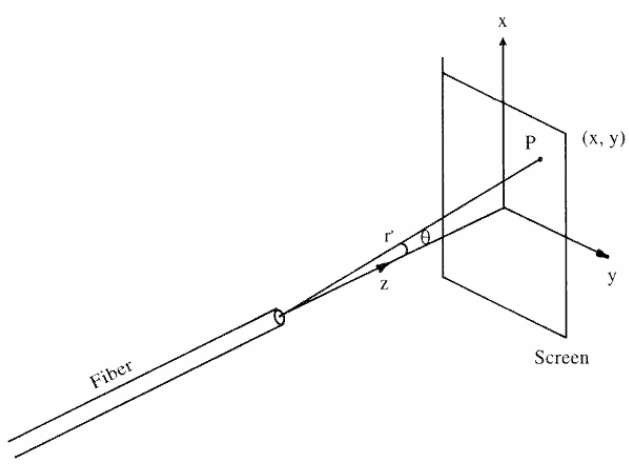
\includegraphics[width=0.7\linewidth]{Image/Far_field.png}
    \caption{Geometry for far-field imaging of the fiber output}
    \label{fig:far_field}
\end{figure}

The far-field amplitude $u$ is determined by the Fraunhofer diffraction
integral, which relates the far field to the angular distribution via a
Fourier transform:
\begin{equation}
u = C \int_{-\infty}^{+\infty} \int_{-\infty}^{+\infty}
\psi(x', y') e^{ik_0(lx' + my')} dx' dy'
\end{equation}

Here, $l = \sin\theta \cos\phi$ and $m = \sin\theta \sin\phi$ are direction
cosines. Due to cylindrical symmetry, we evaluate the distribution along
the $x$-axis ($\phi = 0$), simplifying the kernel to $e^{ik_0 x' \sin\theta}$.
Substituting into the above:

\begin{equation}
u(\theta) = AC \int_{-\infty}^{+\infty} e^{-y'^2/w^2} dy'
\int_{-\infty}^{+\infty} e^{-x'^2/w^2} e^{ik_0 x' \sin\theta} dx'
\end{equation}

Using the Gaussian integral identity:
\begin{equation}
\int_{-\infty}^{+\infty} e^{-px^2 + qx} dx = \sqrt{\frac{\pi}{p}} \,
e^{\frac{q^2}{4p}}
\end{equation}

both integrals evaluate to:
\begin{equation}
u(\theta) = AC (\sqrt{\pi} w)
\left( \sqrt{\pi} w \exp\left[ -\frac{k_0^2 \sin^2\theta}{4/w^2} \right] \right)
= AC \pi w^2 \exp\left( -\frac{k_0^2 w^2 \sin^2\theta}{4} \right)
\end{equation}

The corresponding far-field intensity distribution is:
\begin{equation}
I(\theta) = I(0) \exp\left( -\frac{k_0^2 w^2 \sin^2\theta}{2} \right)
\end{equation}

This is a Gaussian in $\sin\theta$, confirming that the far-field pattern of
a single-mode fiber is also Gaussian — a direct consequence of the Fourier-transform
relationship between near and far fields.

The angle $\theta_e$ at which the far-field intensity falls to $1/e^2$ of the
on-axis value satisfies:
\begin{equation}
\sin\theta_e = \frac{2}{k_0 w} = \frac{\lambda_0}{\pi w}
\end{equation}

Rearranging, the beam waist is directly obtained from the measured $\theta_e$:
\begin{equation}
\boxed{w = \frac{\lambda_0}{\pi \sin\theta_e}}
\end{equation}

\subsection{Coupling Efficiency and Insertion Loss}
The efficiency of the power transfer from the laser source into the fiber is quantified using the measured input power ($P_{in}$) and output power ($P_{out}$). The \textbf{coupling efficiency} $\eta$ is given by:
\begin{equation}
    \eta = \frac{P_{out}}{P_{in}}
\end{equation}
To express this in a standard logarithmic scale, the \textbf{insertion loss} ($L$) is calculated in decibels (dB):
\begin{equation}
    L \, (\text{dB}) = -10 \log_{10} \left( \frac{P_{out}}{P_{in}} \right)
\end{equation}

%%%%%%%%%%%%%%%%%%%%%%%%%%%%%%%%%%%%%
\section{Procedure}
The experiment begins with the precise alignment of the laser beam to ensure efficient coupling into the optical fibre. Initially, the fibre mount is removed and the beam is aligned using two mirrors so that it travels parallel to the optical bench. The alignment is carried out using the \textbf{near–near, far–far method}, where adjustments to the mirror closer to the laser (near mirror) affect the beam position at points farther away, while adjustments to the far mirror influence the beam position near it. By iteratively adjusting the horizontal and vertical screws of the mirrors and checking the beam height and position at different locations along the optical path, a uniform and straight beam propagation is achieved.

\begin{figure}[H]
    \centering
    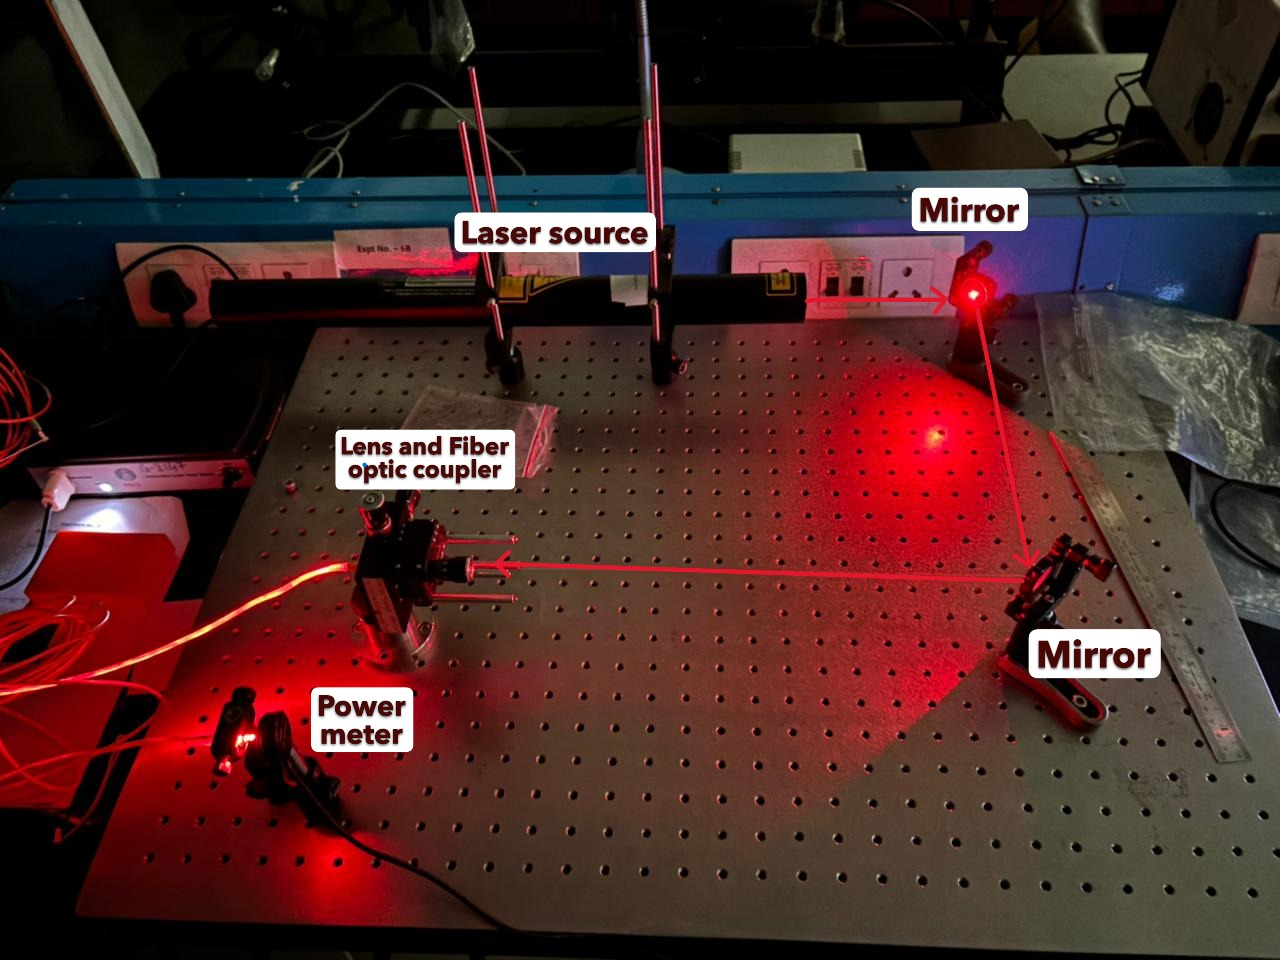
\includegraphics[width=0.7\linewidth]{Image/optical fibre set up.JPG.jpeg}
    \caption{Setup for Fibre optics}
    \label{fig:setup1}
\end{figure}


Once the beam is properly aligned, the fibre optic coupler with the aspheric lens is introduced into the setup. The beam is carefully directed through the centre of the lens to ensure proper focusing into the fibre core. For initial alignment, a multimode fibre is used due to its larger core diameter, making light coupling easier. The lens position is adjusted using a translation stage to maximise the output power, thereby optimising the quantity of transmitted information.

After achieving optimal output with the multimode fibre, it is replaced with a single-mode fibre. Since single-mode fibres are more sensitive to alignment, fine adjustments are required. At this stage, the \textbf{beam walking technique} is employed to improve the coupling efficiency. In this method, the output power is deliberately reduced by adjusting one mirror (typically the far mirror), and then recovered or increased by adjusting the other mirror (near mirror) in a controlled manner. This process is repeated in both horizontal and vertical directions to ensure that the beam is incident normally on the lens and is properly focused into the fibre core without angular misalignment.

To study the quality of information, the intensity profile of the laser beam is first recorded without the fibre using a CCD camera and analysed using image processing software. The procedure is then repeated for the multimode fibre, where multiple propagation modes produce a complex intensity distribution, and for single-mode fibres, where a Gaussian-like profile is observed. All measurements, images, and intensity distributions are systematically recorded and analysed using ImageJ software.

\begin{figure}[H]
    \centering
    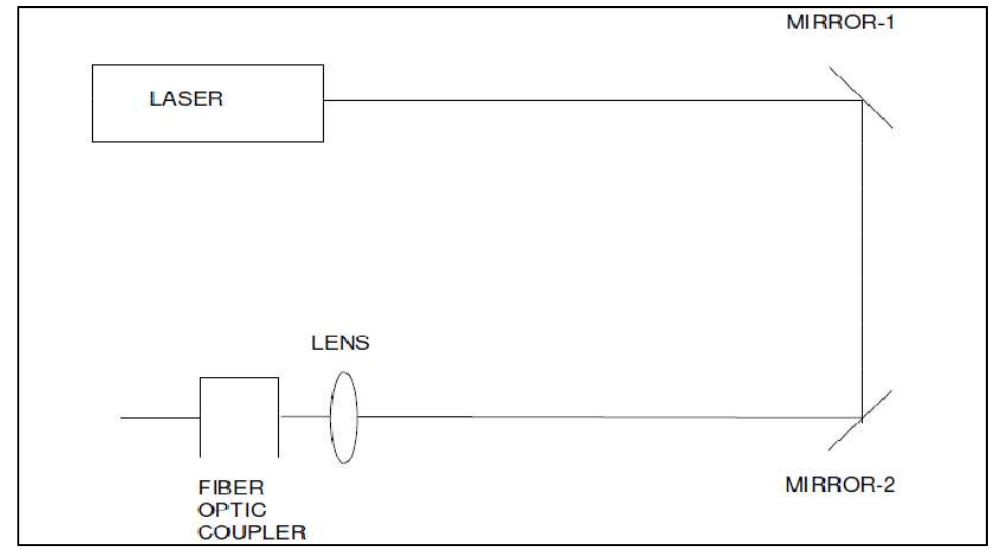
\includegraphics[width=0.6\linewidth]{Image/setup2.png}
    \caption{Schematic diagram of the experimental arrangement}
    \label{fig:setup2}
\end{figure}

%%%%%%%%%%%%%%%%%%%%%%%%%%%%%%%%%%%%%
\section{Plots} 
Based on the procedure mentioned we had set the optical table and did the experiment with the single and multimode lasers. These are following figures of intensity profiles of the single and multimode lasers. 
\begin{figure}[H]
    \centering
    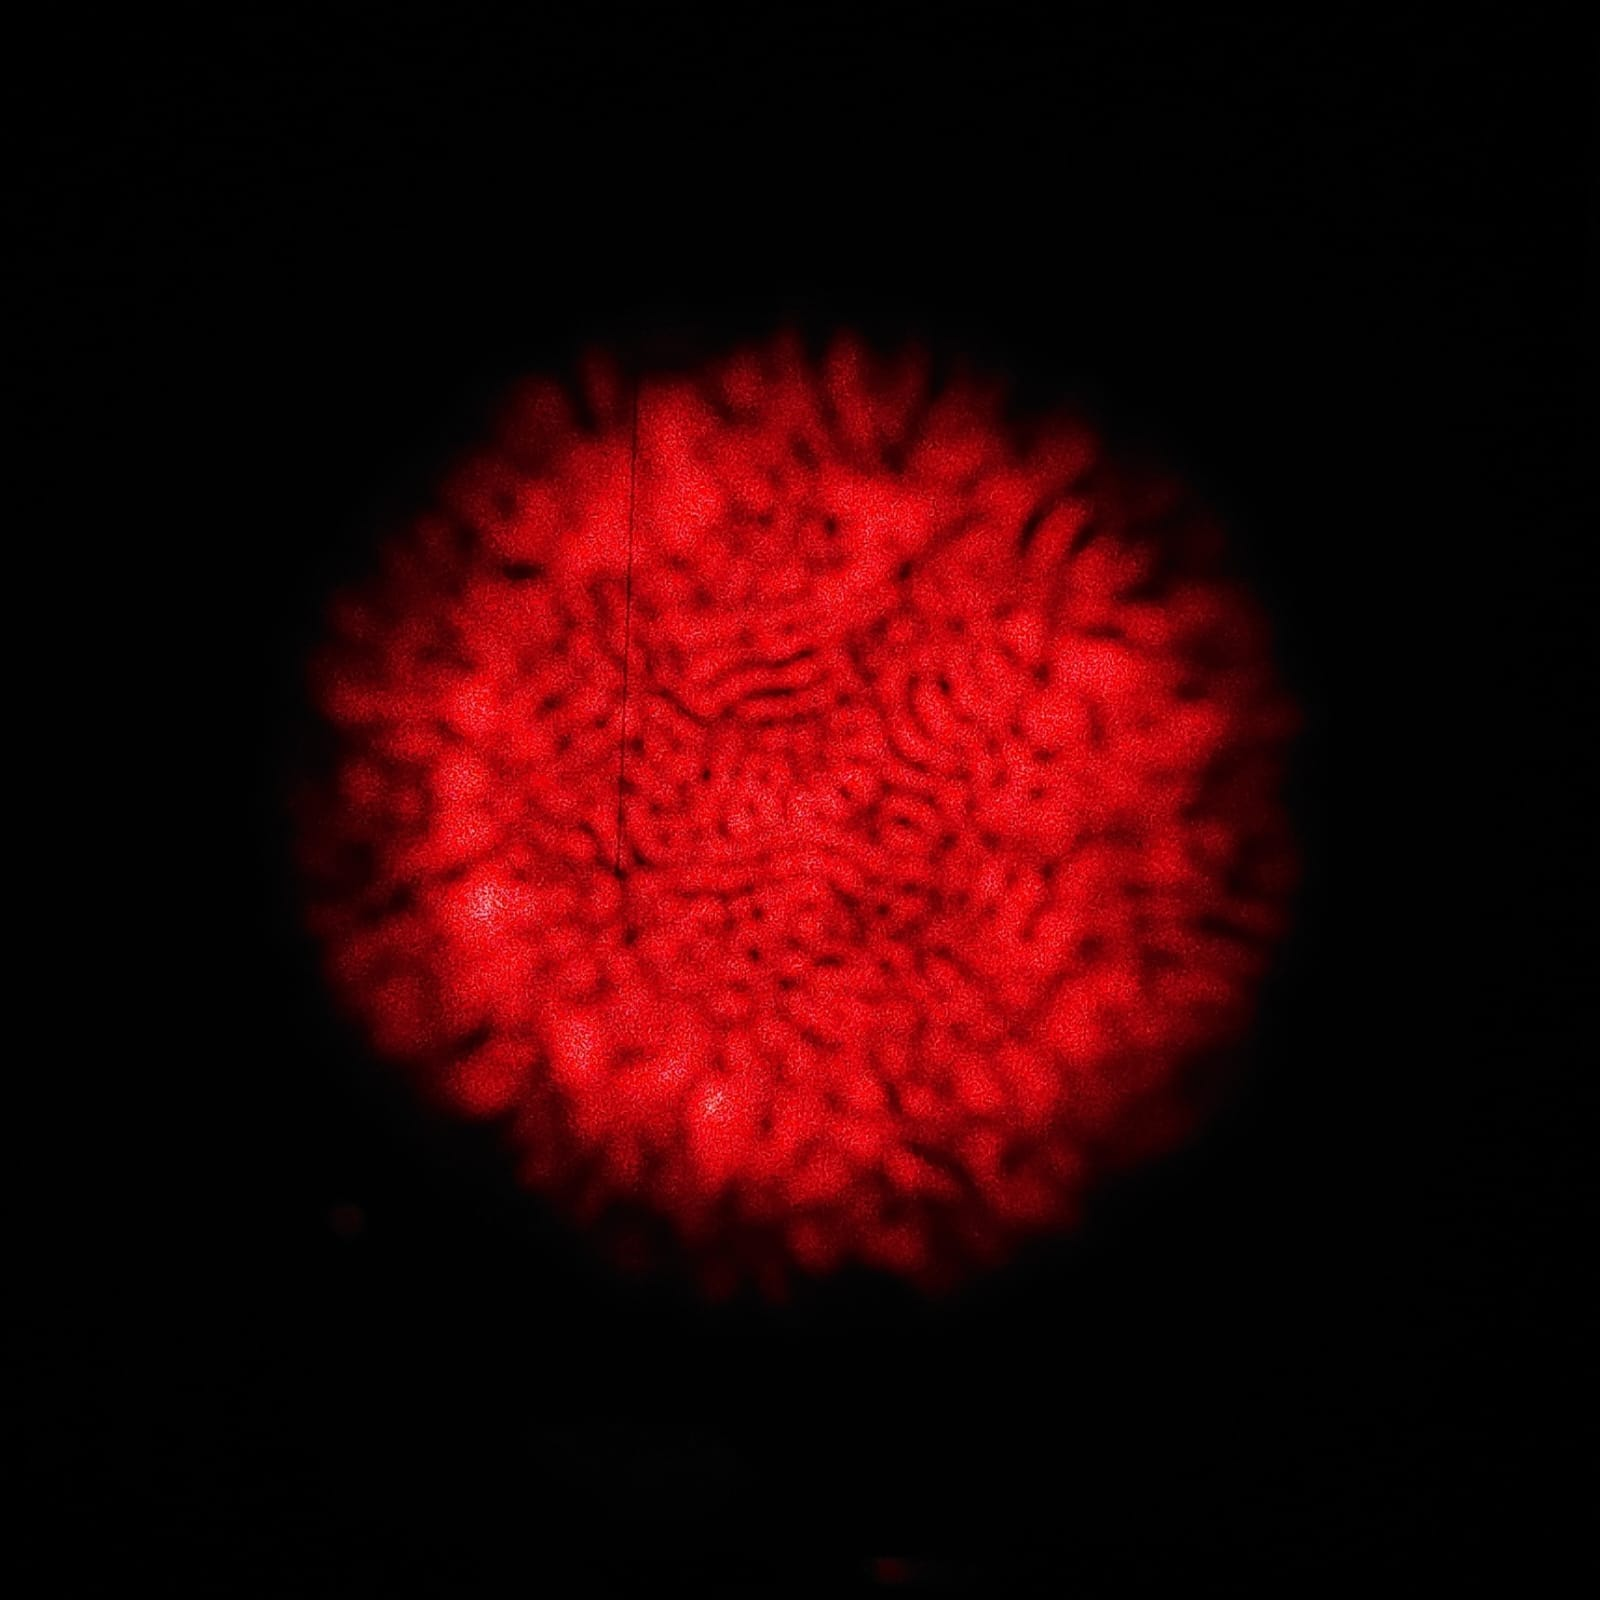
\includegraphics[width=0.5\linewidth]{Image/multi_act.jpeg}
    \caption{Multi Mode fibre Output}
    \label{fig:Muti_mode_out}
\end{figure}

\begin{figure}[H]
    \centering
    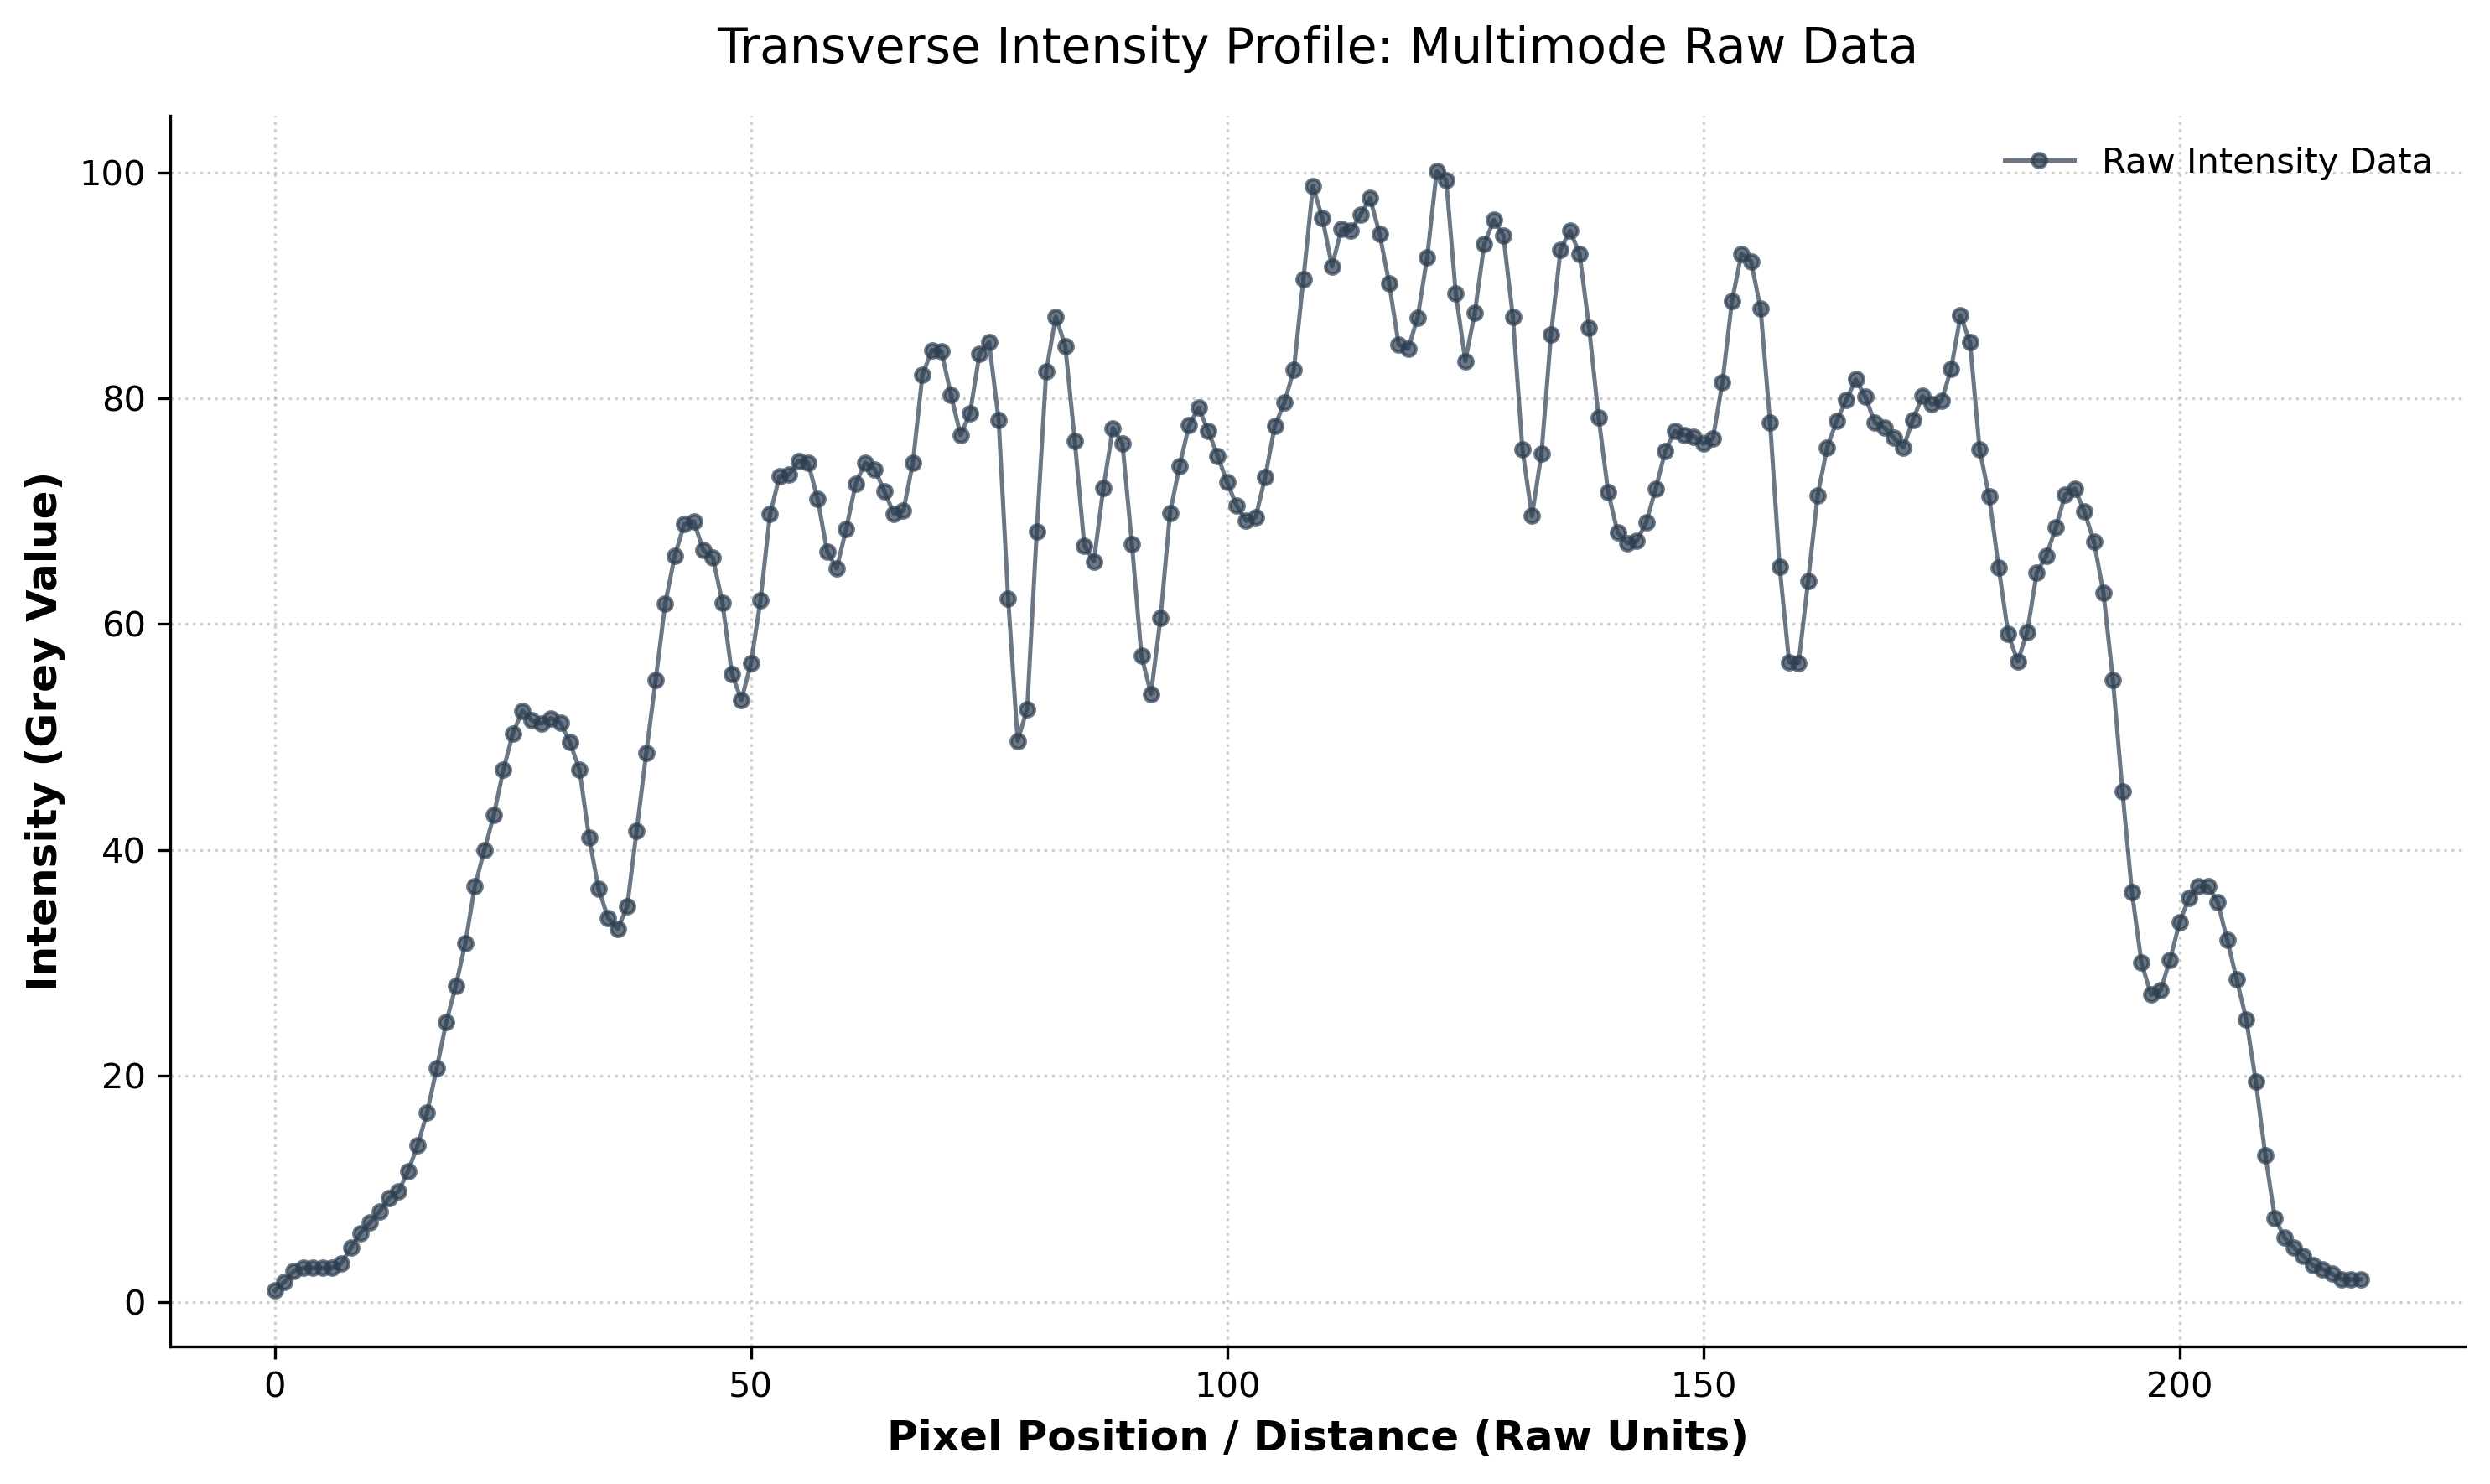
\includegraphics[width=0.7\linewidth]{Image/multimode_raw_scatter_line.png}
    \caption{Multimode Fibre Intensity Profile}
    \label{fig:placeholder}
\end{figure}
\begin{figure}[H]
    \centering
    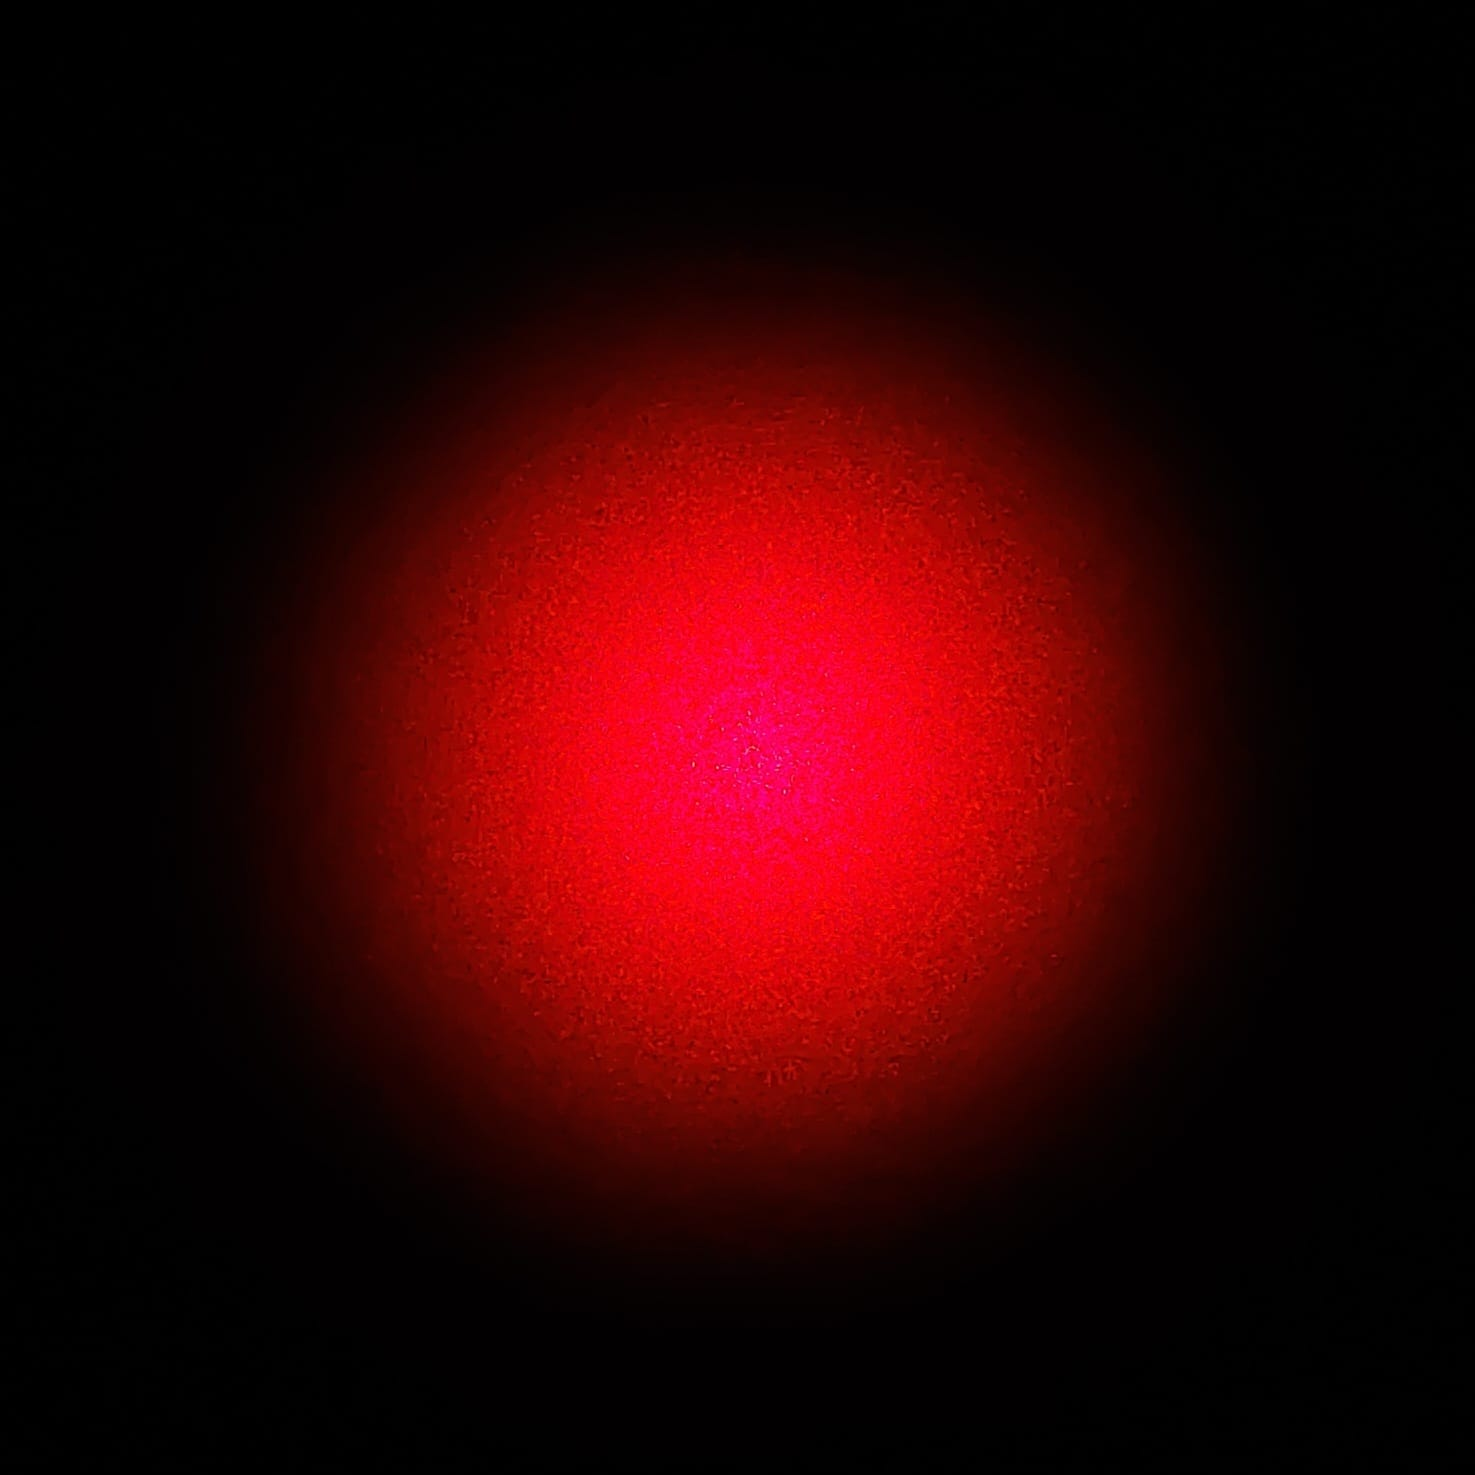
\includegraphics[width=0.4\linewidth]{Image/single_actual.jpeg}
    \caption{Single Mode Fibre (600-800 nm) Output}
    \label{fig:pSingle_mode_out}
\end{figure}

\begin{figure}[H]
    \centering
    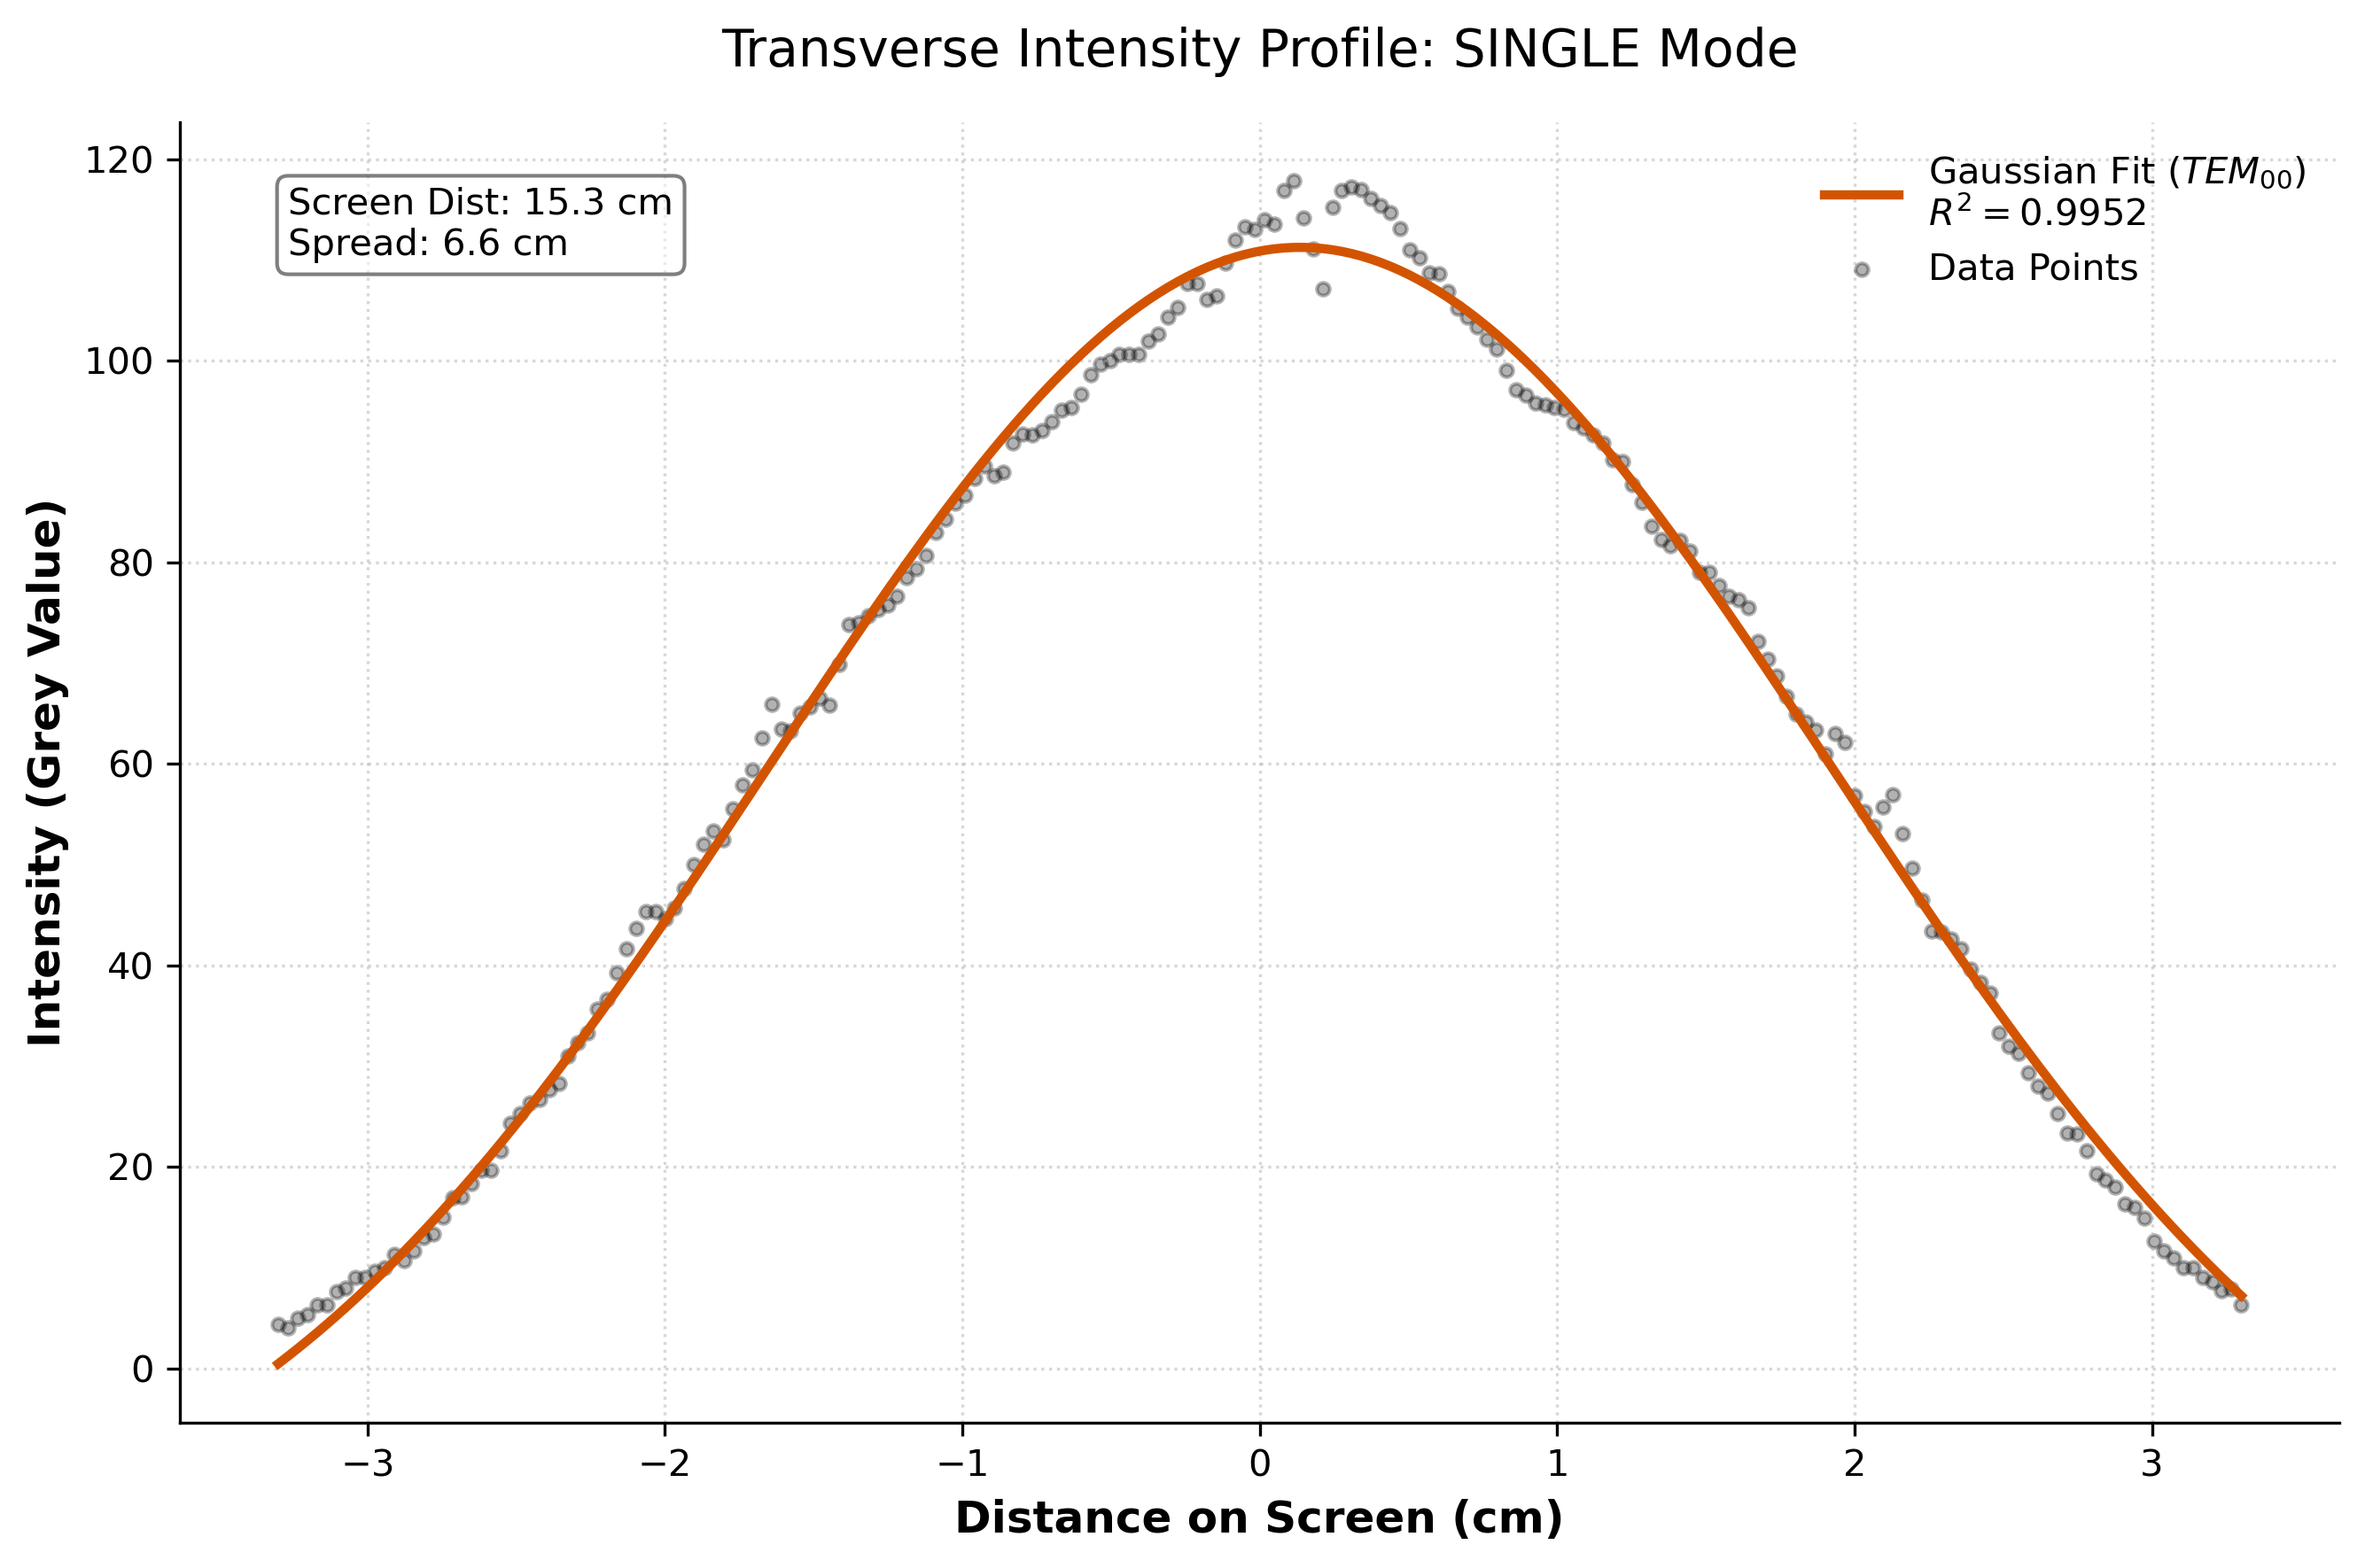
\includegraphics[width=0.65\linewidth]{Image/fiber_profile_single.png}
    \caption{Single Mode Fibre Intensity Profile}
    \label{fig:Single_mode_int}
\end{figure}
%%%%%%%%%%%%%%%%%%%%%%%%%%%%%%%%%%%%%
\section{Calculations and Results}
To characterize the single-mode fiber, we extract the beam radius on the screen, $w_s$, from our Gaussian curve fit. This parameter represents the radial distance where the transmitted intensity falls to $1/e^2$ of its peak value. Using our experimental values---laser wavelength $\lambda = 650$~nm ($6.5 \times 10^{-5}$~cm), screen distance $d = 15.3$~cm, and the extracted beam radius $w_s = 3.0530$~cm---we can directly compute the fundamental properties of the fiber.

\begin{figure}[H]
    \centering
    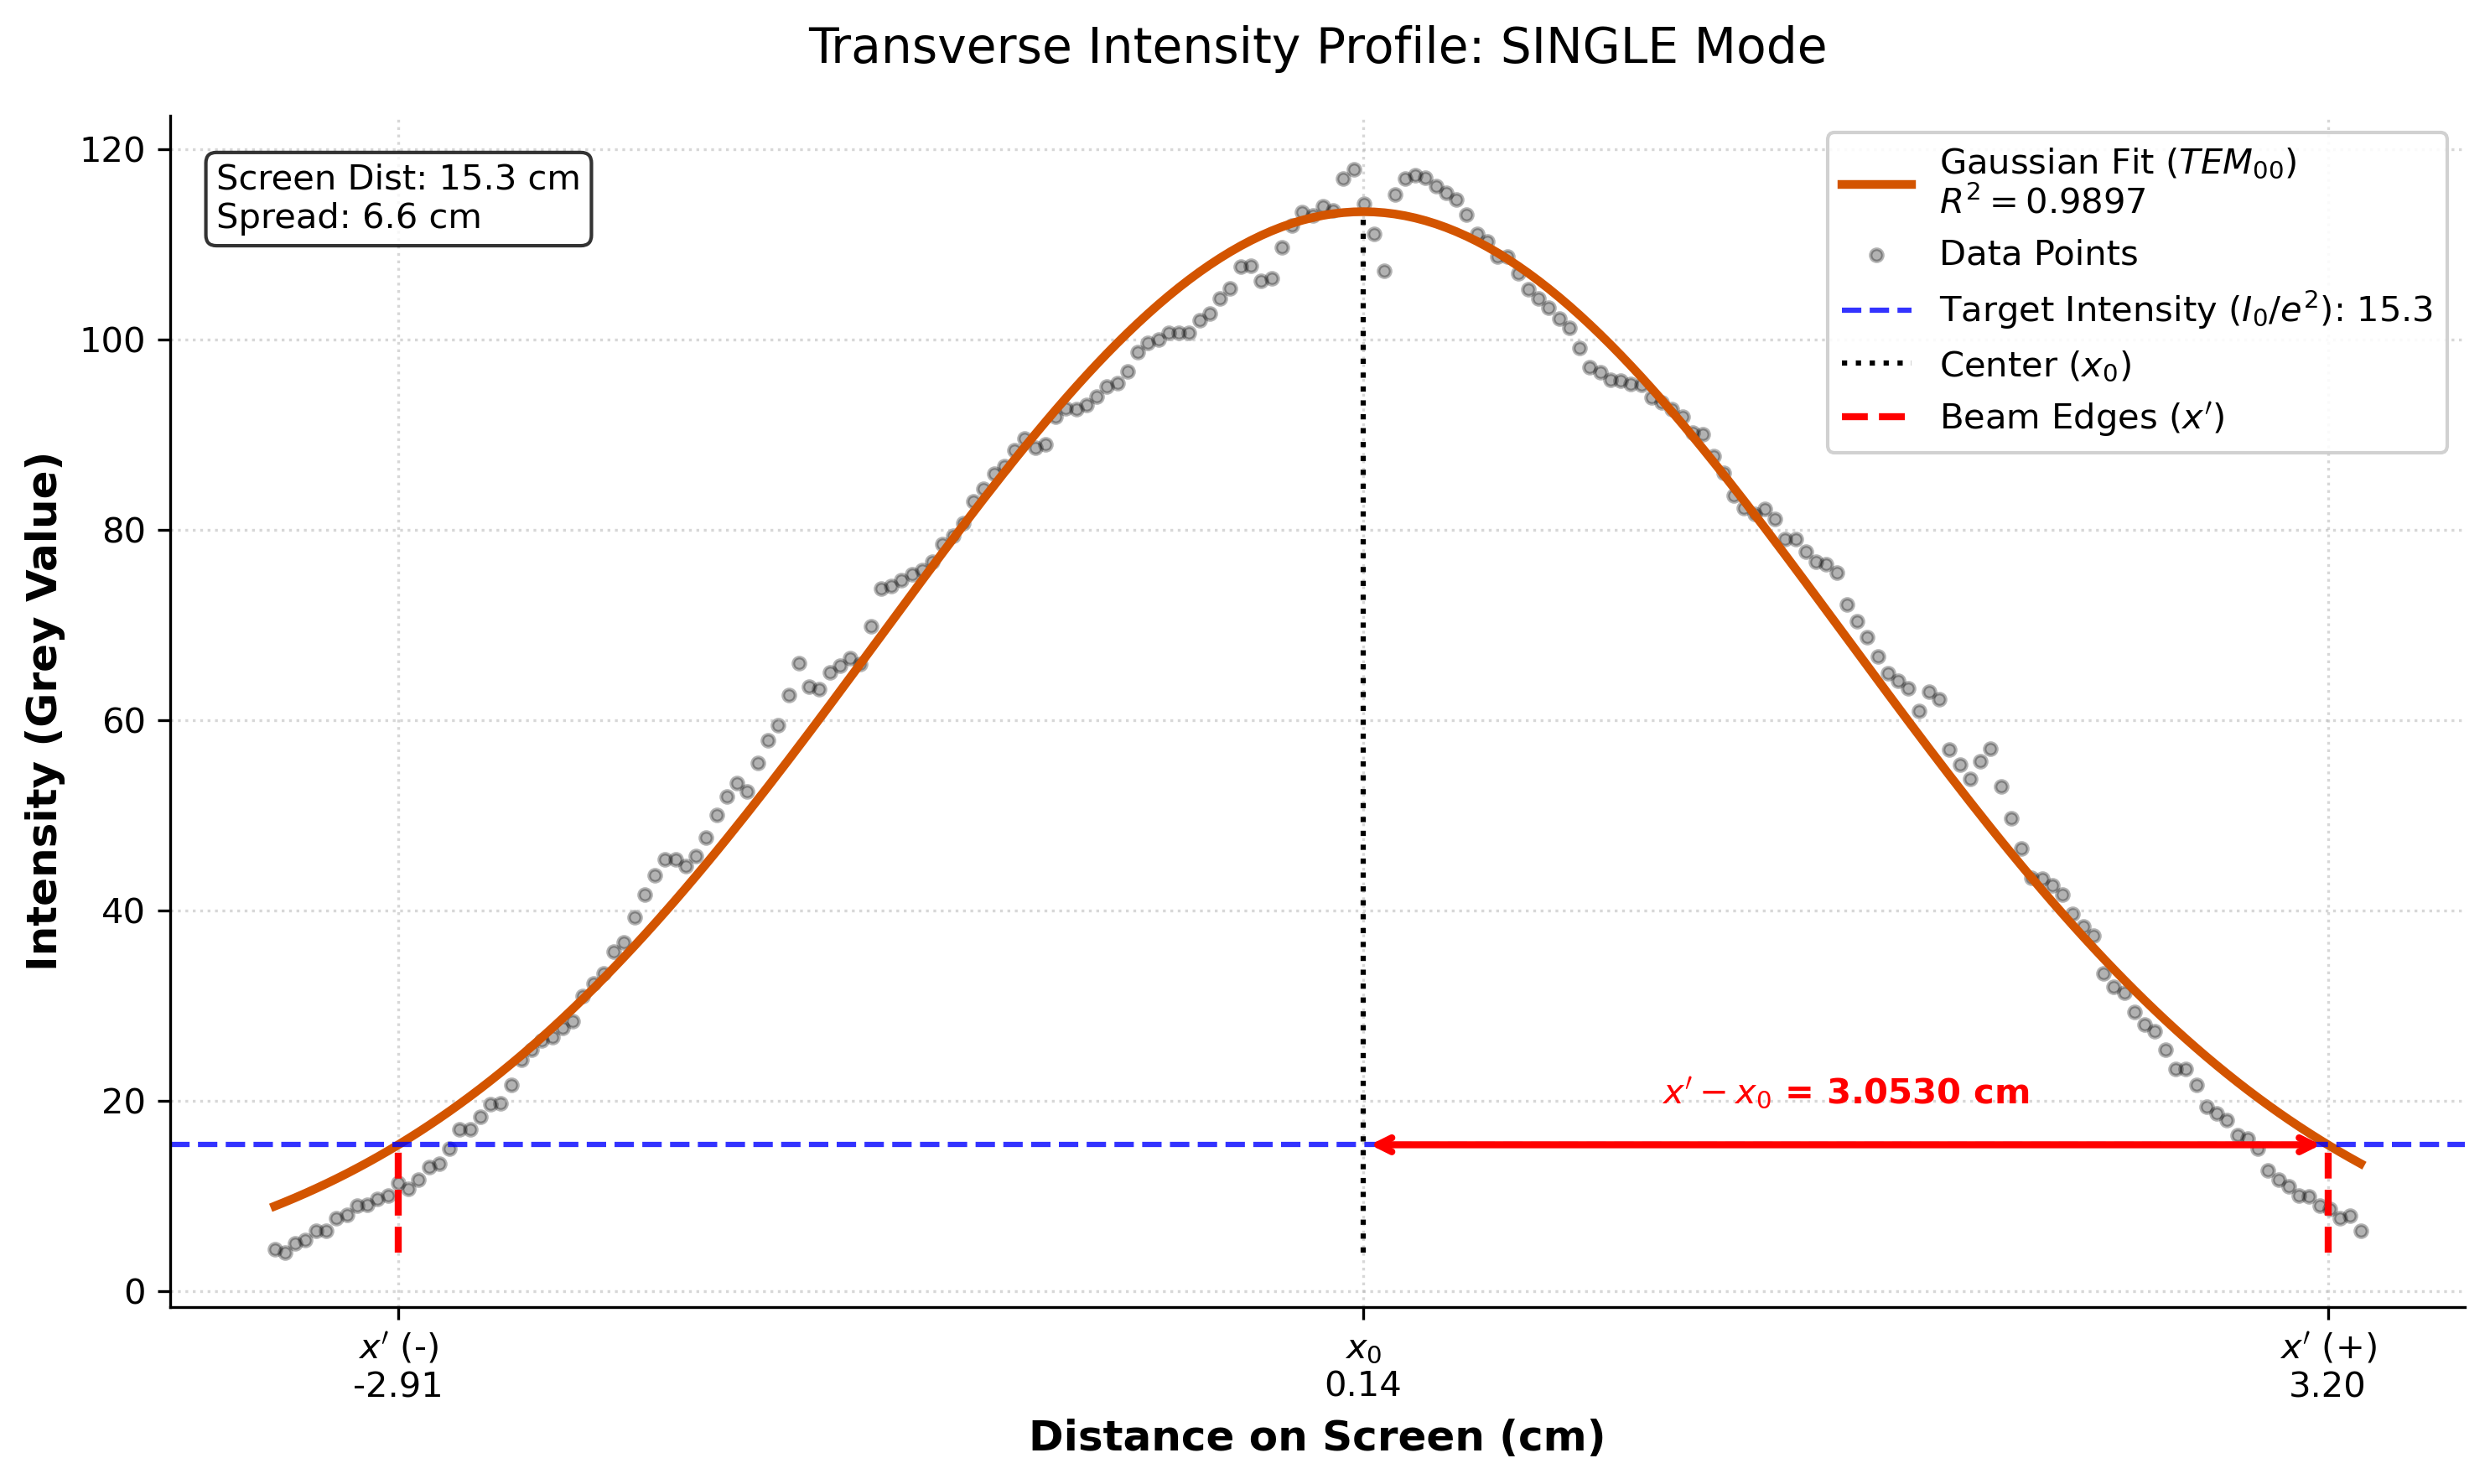
\includegraphics[width=0.7\linewidth]{Image/fiber_profile_single_gauss.png}
    \caption{Determination of $w_s$}
    \label{fig:placeholder}
\end{figure}
\subsection{Numerical Aperture and Divergence}
As the beam exits the fiber, it expands. We find the Numerical Aperture (NA) directly from the exact physical geometry of the far-field spread:
\begin{equation}
    NA = \sin(\theta_e) = \frac{w_s}{\sqrt{w_s^2 + d^2}}
\end{equation}
Plugging in our measurements:
\begin{equation}
    NA = \frac{3.0530}{\sqrt{(3.0530)^2 + (15.3)^2}} \approx 0.1957
\end{equation}
This gives a half-divergence angle of $\theta_e = \arcsin(0.1957) \approx 11.28^\circ$.

\subsection{Near-Field Beam Waist and Mode Field Diameter}
To find the near-field beam waist ($w_0$) at the fiber tip, we use the exact formulation derived from the diffraction limit, which links $w_0$ directly to the NA without relying on small-angle approximations:
\begin{equation}
    w_0 = \frac{\lambda}{\pi \sin\theta_e} = \frac{\lambda}{\pi NA}
\end{equation}
Substituting our values:
\begin{equation}
    w_0 = \frac{6.5 \times 10^{-5} \, \mathrm{cm}}{\pi (0.1957)} \approx 1.057 \times 10^{-4} \, \mathrm{cm} = 1.057 \, \mu\mathrm{m}
\end{equation}
The Mode Field Diameter (MFD) is simply twice this beam waist, defining the total spatial extent of the fundamental $\mathrm{LP}_{01}$ mode:
\begin{equation}
    MFD = 2w_0 = 2(1.057 \, \mu\mathrm{m}) = 2.115 \, \mu\mathrm{m}
\end{equation}

\subsection{Summary of Parameters}
Table \ref{tab:smf_params} summarizes the optical properties derived from our spatial profile.

\begin{table}[H]
\centering
\caption{Calculated Optical Properties for Single-Mode Fiber ($\lambda = 650$ nm)}
\vspace{0.2cm}
\begin{tabular}{|l|c|c|}
\toprule
\textbf{Parameter} & \textbf{Value} & \textbf{Unit} \\ \midrule
Peak Center ($x_0$) & 0.1400 & cm \\
Beam Radius on Screen ($w_s$) & 3.0530 & cm \\
Numerical Aperture ($NA$) & 0.1957 & --- \\
Far-field Divergence ($\theta_e$) & 11.28 & degrees \\
Near-field Beam Waist ($w_0$) & 1.057 & $\mu$m \\
Mode Field Diameter ($MFD$) & 2.115 & $\mu$m \\ \bottomrule
\end{tabular}
\label{tab:smf_params}
\end{table}

\subsection{Coupling Coefficient Analysis}
The coupling coefficient, $\eta$, defines the efficiency of the laser-to-fiber interface and is calculated as the ratio of the output power to the incident laser power ($P_{inc} = 58$~mW). 

For the multimode fiber ($P_{out} = 54$~mW):
\begin{equation}
    \eta_{MM} = \frac{54}{58} \approx 0.9310 \quad (93.10\%)
\end{equation}

For the single-mode fiber ($P_{out} = 51$~mW):
\begin{equation}
    \eta_{SM} = \frac{51}{58} \approx 0.8793 \quad (87.93\%)
\end{equation}
%%%%%%%%%%%%%%%%%%%%%%%%%%%%%%%%%%%%%
\section{Error Analysis}

In any optical setup, physical measurements are subject to precision limits. The screen distance ($d = 15.3$~cm) and the extracted beam radius ($w_s = 3.0530$~cm) both carry an estimated uncertainty of $\Delta d = 0.1$~cm and $\Delta w_s = 0.1$~cm, respectively. These arise primarily from manual alignment tolerances and pixel-to-centimeter calibration limits. To determine how these geometric uncertainties propagate into our final optical parameters, we employ the method of logarithmic differentiation.

\subsection{Uncertainty in Numerical Aperture ($\sin\theta_e$)}
The physical Numerical Aperture is defined by the exact far-field geometry:
\begin{equation}
    \sin(\theta_e) = \frac{w_s}{\sqrt{w_s^2 + d^2}}
\end{equation}
To find the fractional uncertainty, we first take the natural logarithm of both sides:
\begin{equation}
    \ln(\sin\theta_e) = \ln(w_s) - \frac{1}{2}\ln(w_s^2 + d^2)
\end{equation}
Taking the differential and grouping variables by their respective differentials yields the maximum possible uncertainty (worst-case scenario):
\begin{equation}
    \frac{\Delta(\sin\theta_e)}{\sin\theta_e} = \left| \frac{d^2}{w_s(w_s^2 + d^2)} \right| \Delta w_s + \left| \frac{d}{w_s^2 + d^2} \right| \Delta d
\end{equation}
Substituting our updated experimental values ($w_s = 3.0530$~cm, $d = 15.3$~cm, $\Delta w_s = 0.1$~cm, $\Delta d = 0.1$~cm):
\begin{equation}
    w_s^2 + d^2 = (3.0530)^2 + (15.3)^2 \approx 243.41
\end{equation}
\begin{equation}
    \frac{\Delta(\sin\theta_e)}{\sin\theta_e} = \left( \frac{234.09}{3.0530 \times 243.41} \right)(0.1) + \left( \frac{15.3}{243.41} \right)(0.1)
\end{equation}
\begin{equation}
    \frac{\Delta(\sin\theta_e)}{\sin\theta_e} \approx (0.3149)(0.1) + (0.0629)(0.1) = 0.0315 + 0.0063 = 0.0378
\end{equation}
This calculation reveals a relative error of roughly $3.78\%$. Multiplying this by our previously calculated NA value ($\sin\theta_e = 0.1957$):
\begin{equation}
    \Delta(\sin\theta_e) = 0.1957 \times 0.0378 \approx 0.0074
\end{equation}
Thus, our final Numerical Aperture is reported as $0.1957 \pm 0.0074$.

\subsection{Uncertainty in Near-Field Beam Waist ($w_0$)}
To find the uncertainty in the near-field beam waist ($w_0$), we use the diffraction limit relationship:
\begin{equation}
    w_0 = \frac{\lambda}{\pi \sin\theta_e}
\end{equation}
Taking the differentials to find the maximum absolute error yields a direct relationship between the relative uncertainties:
\begin{equation}
    \frac{\Delta w_0}{w_0} = \frac{\Delta(\sin\theta_e)}{\sin\theta_e}
\end{equation}
Because the relative uncertainty of $\sin\theta_e$ was computed as $0.0378$ (or $3.78\%$), we substitute this directly:
\begin{equation}
    \frac{\Delta w_0}{w_0} = 0.0378
\end{equation}
Applying this fractional error to our calculated beam waist value of $w_0 = 1.057 \, \mu\mathrm{m}$:
\begin{equation}
    \Delta w_0 = 1.057 \, \mu\mathrm{m} \times 0.0378 \approx 0.040 \, \mu\mathrm{m}
\end{equation}
Therefore, accounting for propagated geometric measurement errors, the final near-field beam waist is $1.057 \pm 0.040 \, \mu\mathrm{m}$.


%%%%%%%%%%%%%%%%%%%%%%%%%%%%%%%%%%%%%
\section{Sources of Error}

\begin{itemize}

\item \textbf{Alignment Errors:}  
Imprecise alignment of the mirrors, aspheric lens, and fibre coupler can significantly reduce coupling efficiency. Even slight deviations from optimal alignment prevent the beam from entering the fibre core properly.

\item \textbf{Angular Misalignment at Fibre Input:}  
If the laser beam is not incident normally on the fibre end, it can lead to inefficient coupling and excitation of higher-order modes in single-mode fibres, distorting the expected Gaussian profile.

\item \textbf{Beam Walking and Mirror Adjustment Errors:}  
Improper implementation of beam walking or incorrect use of mirror screws (mixing horizontal and vertical adjustments) can disturb alignment and reduce output power.

\item \textbf{Laser Source Instability:}  
Fluctuations in laser output power or wavelength during the experiment can affect both intensity distribution and power measurements.

\item \textbf{Temperature Variations:}  
Changes in ambient temperature may cause thermal expansion of optical components and slight variations in refractive indices, thereby affecting numerical aperture and light propagation.

\item \textbf{Fibre Imperfections:}  
Defects, impurities, or micro-voids in the fibre core can cause scattering and distortion of the transmitted beam.

\item \textbf{Mechanical Stress on Fibre:}  
Bending or improper handling of the fibre can induce stress birefringence, leading to phase differences between modes and instability in the observed intensity pattern.

\item \textbf{Contamination of Optical Components:}  
Dust particles, fingerprints, or dirt on lenses or fibre end faces can reduce transmission efficiency and introduce unwanted distortions.

\item \textbf{CCD Camera Saturation:}  
If the beam intensity exceeds the dynamic range of the CCD, pixel saturation occurs, leading to a flattened intensity profile and inaccurate beam waist estimation.

\item \textbf{Background Noise and Ambient Light:}  
External light and electronic noise in the detector reduce the signal-to-noise ratio, affecting the accuracy of intensity measurements and curve fitting.

\end{itemize}

%%%%%%%%%%%%%%%%%%%%%%%%%%%%%%%%%%%%%
\section{Discussion}
\label{sec:discussion}

\begin{itemize}

\item \textbf{Discussion on fibre}  
The propagation of light within the studied fibers can be understood through the duality of the ray and wave models. The ray model provides an intuitive visualization based on \textbf{Total Internal Reflection (TIR)}, where light is confined to the core as long as the incident angle exceeds the critical angle. However, the wave model is necessary for a rigorous description, as it treats light as an electromagnetic field governed by Maxwell’s equations. This lead to the formation of discrete guided modes due to constructive interference. In our observations, near-axial propagation corresponds to the fundamental $LP_{01}$ mode, while steeper injection angles excite higher-order modes, such as the $LP_{11}$ distribution seen in the multimode fiber.

\item \textbf{Connection with HG Modes:}  
Under the paraxial approximation, LP modes can be approximated by \textbf{Hermite--Gaussian (HG) modes}. Thus, $LP_{01} \approx HG_{00}$ (Gaussian profile), while higher-order LP modes resemble $HG_{10}$ or $HG_{01}$. This explains why the observed beam profiles match Gaussian and multi-lobed patterns.

\item \textbf{Role of V-number:}  
The number of supported modes is governed by the \textbf{$V$-number}.  
\begin{itemize}
    \item For $V < 2.405$, only the fundamental mode propagates (single-mode fibre).
    \item For large $V$, multiple modes are supported (multimode fibre).
\end{itemize}
This was confirmed experimentally, as the single-mode fibre produced a clean Gaussian profile, while the multimode fibre exhibited complex intensity distributions.

\item \textbf{Power vs Quality Trade-off:}  
The multimode fibre showed higher output power due to its larger \textbf{numerical aperture (NA)} and core size, allowing it to accept light over a wider angular range. However, this resulted in \textbf{modal dispersion} and distorted intensity profiles. In contrast, the single-mode fibre preserved beam quality but had lower coupling efficiency.

\item \textbf{Mode Superposition and LG Modes:}  
Hermite--Gaussian modes can be expressed as superpositions of \textbf{Laguerre--Gaussian (LG) modes}, which have an azimuthal phase dependence $e^{\pm i\ell\phi}$. For example, the $HG_{10}$ mode can be written as a combination of $LG_{+1}$ and $LG_{-1}$ modes.

\item \textbf{Geometric (Berry) Phase Effect:}  
A key observation was the rotation of the output intensity pattern when the mirror alignment was slightly changed. This arises due to the \textbf{geometric phase}, where the phase of the optical field depends on its evolution in parameter space rather than path length. Even if we twist the optical fibre then also we can see the pattern changes.
This provides an experimental demonstration of \textbf{Berry phase in optical systems}.
\end{itemize}
The experiment demonstrates that optical fibres act as both waveguides and information carriers. The \textbf{output power represents the quantity of information}, while the \textbf{intensity distribution represents the quality}. Efficient communication requires a balance between these two aspects.

\subsection{Mitigation of Experimental Errors}
To ensure the integrity of these results, several steps were taken to mitigate the sources of error identified previously. Mechanical instabilities and alignment drifts were minimized by using high-precision \textbf{kinematic mounts} and performing the "beam walking" technique to ensure the beam was incident normally on the aspheric lens. To prevent CCD saturation---which would lead to an overestimation of the beam waist---the laser intensity was attenuated, and the camera's exposure settings were carefully calibrated within the linear regime of the sensor.

Environmental and fiber-specific errors, such as thermal drift and bending losses, were addressed by securing the fibers to the optical bench with minimal mechanical tension. This prevents stress-induced birefringence and unwanted phase shifts between modes. Furthermore, by performing the experiment in a temperature-stabilized environment and using high-purity silica fibers, we ensured that the refractive index and numerical aperture remained constant throughout the data acquisition process. These precautions allowed for a high-fidelity comparison between the theoretical Gaussian models and our experimental intensity distributions.
%%%%%%%%%%%%%%%%%%%%%%%%%%%%%%%%%%%%%
\section{Conclusion}

In this experiment, the propagation of laser light through single-mode and multimode optical fibres was successfully studied, demonstrating the fundamental role of total internal reflection in guiding light. The results clearly highlight the distinction between the quantity and quality of information transmission: multimode fibres exhibit higher coupling efficiency due to their larger numerical aperture, while single-mode fibres provide superior beam quality with a well-defined Gaussian intensity profile.

The observed intensity distributions confirmed the theoretical prediction of modal behaviour, where single-mode fibres support only the fundamental mode ($LP_{01} \approx HG_{00}$), whereas multimode fibres support multiple modes leading to complex interference patterns. The dependence of mode structure on the fibre’s $V$-number and coupling conditions was also evident.

Additionally, the experiment demonstrated important optical phenomena such as mode superposition and the geometric (Berry) phase, observed through the rotation of output intensity patterns with changes in mirror alignment.

Overall, the experiment provides a comprehensive understanding of optical fibres as waveguides and information carriers, emphasising the trade-off between power transmission and signal fidelity, which is crucial in modern optical communication systems.
%%%%%%%%%%%%%%%%%%%%%%%%%%%%%%%%%%%%%